
\documentclass{article}


\usepackage[square,numbers]{natbib}
\usepackage{amsmath, epsfig}
\usepackage{amsfonts}
\usepackage{subfigure}
\usepackage{graphicx}
\usepackage{amsfonts}
\usepackage{algorithm}
\usepackage{algorithmic}
\usepackage{easybmat}
\usepackage{footmisc}
\usepackage[usenames,dvipsnames]{color}
\usepackage{subfig}
\renewcommand\algorithmiccomment[1]{// \textit{#1}}
\newcommand{\ignore}[1]{}
\newcommand{\comment}[1]{}
\newcommand{\frank}[1]{\textcolor{red}{\textsf{\emph{\textbf{\textcolor{blue}{#1}}}}}}
\newcommand{\willie}[1]{\textcolor{green}{\textsf{\emph{\textbf{\textcolor{green}{#1}}}}}}
\DeclareMathOperator*{\argmax}{arg\,max}




\begin{document}

\title{New Model}
\author{Willie}
\maketitle
% \mbox{}


\section{Model Specification and Inference}

In the following sections, a particular extraction method for generating data from videos and a specific formulation of the model described in Section~\ref{sec:modeloverview} are given. Inference schemes on this model, which when carried out allow for unsupervised detection and tracking of multiple arbitrary objects, are also described.



\subsection{Extraction}
\label{sec:modelspec_extraction}

We desire an extraction procedure that is as unsophisticated as possible, both to gauge the robustness of this method on potentially noisy extraction data and to ensure that the procedure is applicable to a wide range of videos. For these reasons we choose the method of frame-differencing for all extraction performed in this paper, which involves recording the positions of pixels (or pixel groups) that have exhibited differences in intensity or value in succesive frames beyond a given threshold. In particular, if we let $I_{t}$ be the image difference obtained by subtracting the value of the $(i,j)^{th}$ pixel in video frame $t$ from the value of the $(i,j)^{th}$ pixel in video frame $t+1$, we can define extraction on frame $t$ to be the process that returns the dataset
\begin{equation}
	\Omega_{t} = \{ (i,j) | I_{t}(i,j) > \phi \}
\end{equation}
where $i$ and $j$ respectively denote the two spatial positions of a pixel, and $\phi$ is a given pixel value threshold. Frame differencing on each frame $t =\{1, \ldots, T \}$ yields the dataset
\begin{equation}
	\Omega = \bigcup_{t=1}^{T} \Omega_{t} = \{ (i,j,t) | I_{t}(i,j) > \phi \}
\end{equation}
which is equivalent to data with the baseline features described in Section~\ref{sec:data}.

Frame differencing is unsophisticated, computationally inexpensive, able to be applied to a wide range of static, single-camera videos (note that videos used in the experiments described in the following sections were chosen to be static; moving-camera videos should be used in conjunction with applicable extraction methods that allow for camera movement). We have found that, when correctly implemented, frame differencing is sufficiently general to extract the desired worm-like data clouds from a variety of videos containing multiple moving objects. A few examples of this extraction procedure on single video frames can be found in Figure 3.

\begin{figure}
\centering
{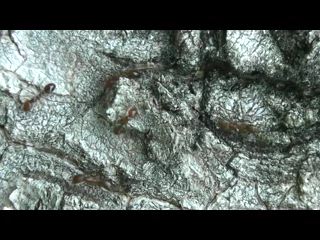
\includegraphics[width=45mm]{antpic2.png}}
%\hspace{2mm}
{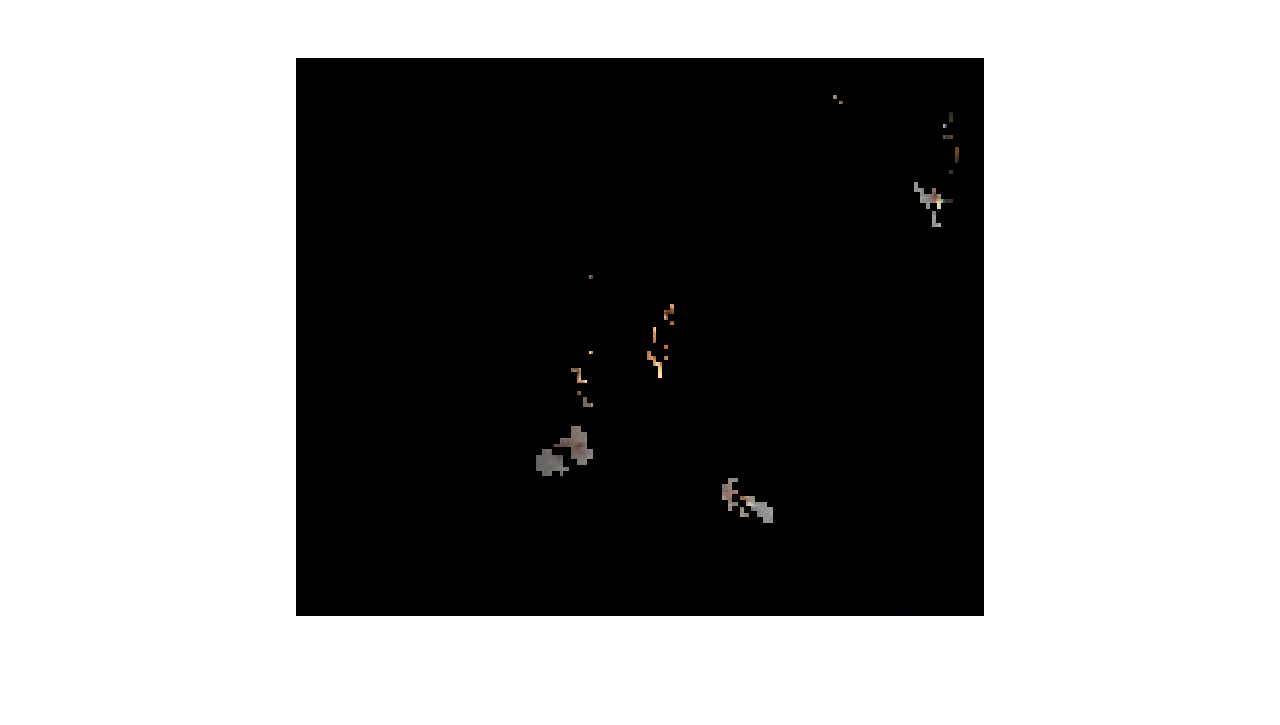
\includegraphics[width=60mm]{frame_diff_ants_1.png}}
\caption{(a.) Frame of a video containing five ants. (b.) Frame differencing extraction results from the same frame \willie{this is just a demo of the type of image i will have here... these aren't actually from the same frame, and also formatting is screwed up)}}
\label{test}
\end{figure}

We furthermore wish to capture the color (or grayscale) value of each pixel and incorporate this color information into our model. For each pixel $x = (i, j, t) \in \Omega$ (defined above), we specify a square, $L$ pixels in length, centered on $(i, j)$, that selects a set of pixels surrounding $\bold{x}$ in frame $t$. We also specify a scalar color value that is able to be computed for each pixel; this value could, for example, be some function of the r-g-b or h-s-v value of a pixel. The color value of each of the selected pixels surrounding $\bold{x}$ is recorded. Afterwards, the set of possible color values (ie the range of color values to which a pixel may be assigned) is partitioned into $V$ bins, and the number of pixels with a color value lying in each of the bins yields a $V$ dimensional vector of `color counts'. We will refer to this extraction technique as `color counting'.

\willie{Show example color-count vector (histogram) for different objects in an image. give more-formal definition like for frame differencing above.}







\subsection{Model Specification for Experiments}
%

\subsubsection{Data}

The frame differencing and color counting extraction outlined above yields a set of data $\bold{X} \subset \mathbb{R}^{2} \times \mathbb{Z}_{+}^{V} \times \mathbb{Z}_{+}$, where each element $\bold{x} \in \bold{X}$ can be written
\begin{equation}
\bold{x} = ( \bold{x}^{s}, \bold{x}^{c}, t ) = ( x^{s_{1}}, x^{s_{2}}, x^{c_{1}}, \ldots, x^{c_{V}}, t )
\end{equation}
where $\bold{x}^{s} \in \mathbb{R}^{2}$ is the two dimensional vector of spatial coordinates,  $\bold{x}^{c} \in \mathbb{Z}_{+}^{V}$ is the $V$ discrete dimensional vector of color counts, and $t \in \mathbb{Z}_{+}$ is the discrete time index. 

In the following experiments, the hue component of a pixel's h-s-v value is recorded from each pixel surrounding a given $\bold{x}^{s}$ in the manner described in Section~\ref{sec:modelspec_extraction} (where we choose $L=5$). Additionally, the set of possible hue values is partitioned into 10 bins, and the number of pixels with a hue value lying in each of the 10 bins is recorded to yield the vector of `color counts' $\bold{x}^{c} = x^{c_{1}}, \ldots, x^{c_{10}}$. Hue is chosen to represent object color since it has been demonstrated in previous work as a simple representation of object appearance that allows for distinct objects to be well differentiated (\willie{cite mckenna, other papers here}).



\subsubsection{Likelihood and Object Appearance Model}

At a given time $t$, we model each $\bold{x} \in \bold{X}$ as a draw from the product of a multivariate normal and multinomial distribution
\begin{equation}
P(\bold{x}|\theta) = \mathcal{N}(\bold{x}^{s} | \boldsymbol{\mu}, \Sigma)  \mathcal{M}n(\bold{x}^{c} | \bold{p})
\end{equation}
where $\theta = \{ \boldsymbol{\mu}, \Sigma, \bold{p} \}$ denote the parameters of a cluster at time $t$, with mean $\boldsymbol{\mu} \in \mathbb{R}^{2}$, covariance matrix $\Sigma \in \mathbb{R}^{2} \times \mathbb{R}^{2}$, and discrete probability vector $\bold{p} = (p_{1}, \ldots, p_{V})$ such that $\sum_{i=1}^{V}p_{i} = 1$. Also, $\mathcal{N}$ denotes the multivariate normal distribution and $\mathcal{M}n$ denotes the multinomial distribution, 

The distribution families assumed to generate each $\bold{x}$ must be justified. Both the multivariate normal and multinomial distributions were chosen because they are sufficiently simple (and well studied) to allow for tractable inference and sufficiently flexible to provide a reasonable approximation to the data gained during extraction. In particular, the multivariate normal distribution over the spatial features $\bold{x}^{s}$ can be thought to represent the shape of each object as an oval; likewise, data generated by each moving object during extraction are often ovular--as noisy extraction procedures cause some smoothing of edges and corners, producing blob-like shapes even when objects are not particularly round--and centered on a given object. Furthermore, this model is justified as the maximum likelihood parameter estimate of a normal distribution corresponds to the least squares fit of data relative to the mean of the distribution. \willie{needs to be said more accurately and explained why this helps.} Modeling the color features $\bold{x}^{c}$ as draws from a multinomial distribution (equivalently, as draws from a product of discrete distributions), is justified since distinct object tend to generate pixels whose hue values are noisy but yield consistent counts in discrete hue bins.



\subsubsection{Base Distribution $\mathbb{G}_{0}$ and Appearance Prior}

$\mathbb{G}_{0}$ denotes the base distribution of the time-dependent Dirichlet process mixture; it also serves as a prior distribution for the parameters $\theta = \{ \boldsymbol{\mu}, \Sigma, \bold{p} \}$ present in the likelihood. We make use of conjugate priors in the base distribution to allow for more efficient computation. Specifically, in the experiments carried out in this paper, a normal-inverse-Wishart prior is placed on the multivariate normal parameters $\{ \boldsymbol{\mu}, \Sigma \}$ , and a Dirichlet prior is placed on the multinomial parameter $ \{  \bold{p}  \} $ (where the normal-inverse-Wishart is a conjugate prior for the multivariate normal component of the likelihood and the Dirichlet is a conjugate prior for the multinomial component). The prior can thus be written
\begin{equation}
\mathbb{G}_{0}(\theta) = \mathcal{N}i\mathcal{W}(\boldsymbol{\mu}, \Sigma | \boldsymbol{\mu}_{0}, k_{0}, v_{0}, \Lambda_{0})  \mathcal{D}ir( \bold{p} | \bold{q}_{0})
\end{equation}
where $\mathcal{N}i\mathcal{W}$ denotes the normal-inverse-Wishart distribution, $\mathcal{D}ir$ denotes the Dirichlet distribution, and the prior has the hyperparameters $\boldsymbol{\mu}_{0}, k_{0}, v_{0}, \Lambda_{0}$ and $\bold{q}_{0}$.  \willie{reference text with good background on NiW and Dir distributions}



\subsubsection{Transition Kernels and Motion Behavior}

We wish to formulate a transition kernel $P(\theta_{t} | \theta_{t-1})$ that provides a reasonable representation of how we expect tracked objects to behave. In the interest of formulating a model with the intention of using it to track arbitrary objects, we do not wish to make many assumptions about the long-term behavior of objects (though transition kernels that incorporate, for example, dynamics could potentially be implemented if one is aware beforehand of an object's behavior).

As described in Section~\ref{sec:gpudpm}, $\mathbb{G}_{0}$ must be the invariant distribution of $P(\theta_{t} | \theta_{t-1})$ in order for the the cluster parameters to remain marginally distributed according to the base distribution. In other words, the transition kernel must satisfy
\begin{equation}
\int \mathbb{G}_{0}(\theta_{t-1})P(\theta_{t} | \theta_{t-1}) d\theta_{t-1} = \mathbb{G}_{0}(\theta_{t})
\end{equation}
for a given cluster $\theta$. One way to achieve this is through the use of auxiliary variables. Auxiliary variables are a set of $M$ variables $\bold{z}_{t} = (z_{t,1}, \ldots, z_{t,M})$ associated with a each cluster $\theta$ at time $t$ that satisfy
\begin{eqnarray}
% P(\theta_{k,t} | \theta_{k,t-1}) = \int P(\theta_{k,t} | \bold{z}_{k,t}) P(\bold{z}_{k,t} | \theta_{k,t-1}) d \bold{z}_{k,t}
P(\theta_{t} | \theta_{t-1}) = \int P(\theta_{t} | \bold{z}_{t}) P(\bold{z}_{t} | \theta_{t-1}) d \bold{z}_{t}  %\\
% P(\theta', \bold{z}_{t}) = p(\bold{z}_{t}|\theta') \mathbb{G}_{0}(\theta')
\end{eqnarray}

In this way, the parameters of a cluster at a given time do not depend directly on their value at the previous time; they are instead dependent upon an intermediate sequence of auxiliary variables chosen to satisfy the above criteria, which allows the cluster parameters at each time step to be marginally distributed according to the base distribution $\mathbb{G}_{0}$.

For each cluster, we introduce $M$ auxiliary variables $z_{t, 1}, \ldots, z_{t, M}$ at time $t$ that are each drawn from the product of a multivariate normal and multinomial when conditioned on the associated cluster parameters $\theta_{t} = \{ \boldsymbol{\mu}_{t}, \Sigma_{t}, \bold{p}_{t} \}$:
\begin{equation}
z_{t, m} | \boldsymbol{\mu}_{t}, \Sigma_{t}, \bold{p}_{t}  \sim  \mathcal{N}(\boldsymbol{\mu}_{t}, \Sigma_{t}) \mathcal{M}n(\bold{p}_{t})   \hspace{15pt}   
\forall m \in \{ 1, \ldots, M \}
\end{equation}
To satisfy the above criteria for auxiliary variables, at each time $t$ we specify the dependencies of a given cluster on its associated set of auxiliary variables by
\begin{equation}
\boldsymbol{\mu}_{t}, \Sigma_{t}, \bold{p}_{t} | \bold{z}_t  \sim  \mathcal{N}i\mathcal{W}(\boldsymbol{\mu}_{M}, k_{M}, v_{M}, \Lambda_{M})  \mathcal{D}ir(\bold{q}_{M})
\end{equation}
where $\boldsymbol{\mu}_{M}, k_{M}, v_{M}, \Lambda_{M},$ and $\bold{q}_{M}$ are parameters given by:
\willie{ran out of time. need to type up updates here.}





\subsubsection{Previous Model Write-up}


For a given object $k$ at video frame $t$, the set of positions of the object's motion points are modeled with a product (over each position dimension) of one-dimensional Gaussians
\begin{equation}
P(x_{t_{i}}^{pos} | \mu_{t, k}, \lambda_{t, k}) = \prod_{d=1}^{D} \mathcal{N}(x_{t_{i}}^{pos_{d}} | \mu_{t, k}^{d}, \lambda_{t, k}^{d})
\end{equation}
where $x_{t_{i}}^{pos} = \{ x_{t_{i}}^{pos_{1}}, \cdots, x_{t_{i}}^{pos_{D}} \}$,  $\mu_{t, k}^{d}$ is the mean of the $k^{th}$ Gaussian at time $t$ for dimension $d$, and $\lambda_{t, k}^{d}$ is the precision of the $k^{th}$ Gaussian at time $t$ for dimension $d$.  Likewise, for a given object $k$ at video frame $t$, the set of color vectors of the object's motion points are modeled with a multinomial
\begin{equation}
P(x_{t_{i}}^{col} | m_{t, k}) = Mult(x_{t_{i}}^{col} | m_{t, k})
\end{equation}
where $x_{t_{i}}^{col} = \{ x_{t_{i}}^{col_{1}}, \cdots, x_{t_{i}}^{col_{V}} \}$, $m_{t,k} = \{ m_{t,k}^{1}, \cdots, m_{t,k}^{V} \}$, $\sum_{v=1}^{V} m_{t, k}^{v} = 1$, and $m_{t,k}^{v}>0 \hspace{8pt} \forall v \in \{ 1, \cdots, V \}$. The likelihood for a motion point observation is thus
\begin{equation}
P(x_{t_{i}} | \mu_{t, k}, \lambda_{t, k}, m_{t, k}) =  Mult(x_{t_{i}}^{col} | m_{t, k})   \prod_{d=1}^{D}  \mathcal{N}(x_{t_{i}}^{pos_{d}} | \mu_{t, k}^{d}, \lambda_{t, k}^{d}) 
\end{equation}

I want to justify distribution families chosen for appearance modeling in this implementation. To include: the edges of an object are detected well with frame differencing, so while extraction data densities aren't necessarily Gaussians with maxima over the targets, they are usually radially centered around the centroids of targets. Furthermore (thing frank said about gaussians and what they do---minimize least squared distance or something).


\subsubsection{Base Distribution $\mathbb{G}_{0}$ and Appearance Prior}
$\mathbb{G}_{0}$ is the base distribution of the underlying time-dependent Dirichlet process mixture; it also serves as a prior distribution for the parameters present in the likelihood. We make use of conjugate priors in the base distribution to allow for more efficient computation. In particular, for an object $k$ at time $t$, we let the prior distribution over the parameters of the motion point position distribution, $\mu_{t, k}$ and $\lambda_{t, k}$, be 
\begin{equation}
\mathbb{G}_{0}^{pos}(\mu_{t, k}, \lambda_{t, k} | \mu_{0}, n_{0}, a, b) = \prod_{d=1}^{D}[\mathcal{N}(\mu_{t, k}^{d} | \mu_{0}, n_{0} \lambda_{t, k}^{d})   Ga(\lambda_{t, k}^{d} | a, b)]
\end{equation}
where $\mu_{0}, n_{0}, a,$ and $b$ are parameters of the base distribution. Furthermore, for object $k$ at time $t$, we let the prior distribuion over the parameters of the motion point color vector distribution be
\begin{equation}
\mathbb{G}_{0}^{col}(m_{t, k} | q) = Dir(m_{t, k} | q)
\end{equation}
where $q = \{ q^{1}, \cdots, q^{V} \}$ is a parameter of the base distribution, where $q^{v}>0 \hspace{8pt} \forall v \in \{ 1, \cdots, V \}$. The base distribution is thus 
\begin{equation}
\mathbb{G}_{0}(\mu_{t, k}, \lambda_{t, k}, m_{t, k} | \mu_{0}, n_{0}, a, b, q) = Dir(m_{t, k} | q)  \prod_{d=1}^{D}[\mathcal{N}(\mu_{t, k}^{d} | \mu_{0}, n_{0} \lambda_{t, k}^{d})   Ga(\lambda_{t, k}^{d} | a, b)]
\end{equation}


\subsubsection*{Transition Kernels and Motion Behavior}
Let $\phi_{t,k}^{pos} = \{ \mu_{t, k}, \lambda{t, k} \}$ and $\phi_{t,k}^{col} = \{ m_{t, k} \}$.  We define two transition kernels, $P(\phi_{t, k}^{pos} | \phi_{t-1, k}^{pos})$ and $P(\phi_{t, k}^{col} | \phi_{t-1, k}^{col})$, which dictate, respectively, the random walk of the motion point position parameters and the motion point color vector parameters over time. The transition kernels must be chosen so that their invariation distributions are $\mathbb{G}_{0}$, i.e. such that the following hold:
\begin{equation}
\int \mathbb{G}_{0}^{pos}(\phi_{t-1, k}^{pos}) P(\phi_{t, k}^{pos} | \phi_{t-1, k}^{pos}) d\phi_{t-1, k}^{pos}  =  \mathbb{G}_{0}^{pos}(\phi_{t, k}^{pos})
\end{equation}
\begin{equation}
\int \mathbb{G}_{0}^{col}(\phi_{t-1, k}^{col}) P(\phi_{t, k}^{col} | \phi_{t-1, k}^{col}) d\phi_{t-1, k}^{col}  =  \mathbb{G}_{0}^{col}(\phi_{t, k}^{col})
\end{equation}



\end{document}
